\PassOptionsToPackage{dvipsnames}{xcolor}
\documentclass[oneside,11pt]{book}
\usepackage{pagecolor}
\usepackage[utf8]{inputenc}
\usepackage[T1]{fontenc}
\usepackage{soul}
\usepackage[margin=1.5in]{geometry}
\usepackage{tcolorbox}
\tcbuselibrary{documentation, skins}
\usepackage{titlesec}

% \setsecnumdepth{subsection}
% \setcounter{tocdepth}{3}
\usepackage{fontawesome5}
\usepackage{censor}
\usepackage{enumitem}
\usepackage{epigraph}
\newcommand{\myepigraphsimpsons}[1]{
  \epigraph{\vspace{-0.2in} \emph{#1}}{\textsc{The Simpsons}}
}

\usepackage{cite}
\usepackage{caption}
\captionsetup{font=small}
\usepackage{graphicx}
\usepackage{pdfpages}
\usepackage{hyperref}
\usepackage{wrapfig}
\setlength\intextsep{0pt} % remove extra space above and below in-line float

\usepackage{booktabs}

\usepackage{tikz}
\usetikzlibrary{positioning,calc,arrows.meta,shapes.geometric}

%\usepackage[dvipsnames]{xcolor}
%\usepackage{anyfontsize}
%\usepackage{sectsty}
%\usepackage[acronym]{glossaries}
%\setacronymstyle{long-short-desc}
%\makeglossaries{}
%\usepackage[makeroom]{cancel}

% boxes
\newtcolorbox{marker}[1][]{enhanced,
  before skip balanced=2mm,after skip balanced=3mm,
  boxrule=0.4pt,left=5mm,right=2mm,top=1mm,bottom=1mm,
  colback=yellow!10,
  sharp corners,rounded corners=southeast,arc is angular,arc=3mm,
  underlay={%
    \path[fill=tcbcolback!80!black] ([yshift=3mm]interior.south east)--++(-0.4,-0.1)--++(0.1,-0.2);
    \path[draw=tcbcolframe,shorten <=-0.05mm,shorten >=-0.05mm] ([yshift=3mm]interior.south east)--++(-0.4,-0.1)--++(0.1,-0.2);
    \path[fill=tcbcolback!80!black,draw=none] (interior.south west) rectangle node{\large\bfseries {#1}} ([xshift=4mm]interior.north west);
    },
  drop fuzzy shadow}

\newenvironment{commentbox}[1][]{
  \small
  \begin{marker}[\faChessPawn{}]
    {\textbf{#1}}
  }{
  \end{marker}
}

\newenvironment{surprisebox}[1][]{
  \small
  \begin{marker}[\faChessKnight{}]
    {\textbf{#1}}
  }{
  \end{marker}
}

\newenvironment{examplebox}[1][]{
  \small
  \begin{marker}[\faChessBishop{}]
    {\textbf{#1}}
  }{
  \end{marker}
}

\newenvironment{questionbox}[1][]{
  \small
  \begin{marker}[\faChessRook{}]
    {\textbf{#1}}
  }{
  \end{marker}
}

\newenvironment{keybox}[1][]{
\small
  \begin{marker}[\faChessQueen{}]
    {\textbf{#1}}
  }{
  \end{marker}
}

\newenvironment{warningbox}[1][]{
  \small
  \begin{marker}[\faChessKing{}]
    {\textbf{#1}}
  }{
  \end{marker}
}

\newcommand{\code}{\texttt}
\renewcommand{\figurename}{Fig.}
\renewcommand{\tablename}{Tab.}
%\def\Section{\S}
\newcommand{\Section}{\textsection}

\renewcommand{\figureautorefname}{Fig.}
\renewcommand{\tableautorefname}{Tab.}
\makeatletter
\renewcommand{\chapterautorefname}{\textsection\@gobble}
\renewcommand{\sectionautorefname}{\textsection\@gobble}
\renewcommand{\subsectionautorefname}{\textsection\@gobble}
\renewcommand{\appendixautorefname}{\textsection\@gobble}

\newcommand*\l@chapterinfo{\@nodottedtocline{0}{0.0em}{1.5em}}
\newcommand*\l@sectioninfo{\@nodottedtocline{1}{1.5em}{2.3em}}
\newcommand*\l@subsectioninfo{\@nodottedtocline{2}{3.8em}{3.2em}}

% Copied from the book class macro `\@dottedtocline`. Removed the dots and page number
\def\@nodottedtocline#1#2#3#4#5{%
  \ifnum #1>\c@tocdepth \else
    \vskip \z@ \@plus.2\p@
    {\leftskip #2\relax \rightskip \@tocrmarg \parfillskip -\rightskip
     \parindent #2\relax\@afterindenttrue
     \interlinepenalty\@M
     \leavevmode
     \@tempdima #3\relax
     \advance\leftskip \@tempdima \null\nobreak\hskip -\leftskip
     {#4}\nobreak
     \leaders\hbox{$\m@th
        \mkern \@dotsep mu\hbox{\,}\mkern \@dotsep
        mu$}\hfill
     \nobreak
     \hb@xt@\@pnumwidth{\hfil\normalfont \normalcolor }%
     \par}%
  \fi}



\makeatother

\newcommand{\chapterinfo}[1]{%
  \phantomsection
  \addcontentsline{toc}{chapterinfo}{\textcolor{black}{\emph{#1}}}%
}
\newcommand{\sectioninfo}[1]{%
  \phantomsection
  \addcontentsline{toc}{sectioninfo}{\textcolor{black}{\emph{#1}}}%
}
\newcommand{\subsectioninfo}[1]{%
  \phantomsection
  \addcontentsline{toc}{subsectioninfo}{\textcolor{black}{\texttt #1}}%
}

\newcommand{\mycomment}[3][\color{blue}]{{#1{{#2}: {#3}}}}
\newcommand{\tvn}[1]{\mycomment{TVN}{#1}}{}
\newcommand{\didi}[1]{\mycomment{Didier}{#1}}{}
\newcommand{\tl}[1]{\mycomment{ThanhLe}{#1}}{}
\newcommand{\xz}[1]{\mycomment{Xiaokuan}{[#1]}}{}
\newcommand{\red}[1]{{\color{red}{#1}}}

\newcommand{\mytitle}{Roars Lab's Handbook}
%\newcommand{\mysubtitle}{A Handbook for Navigating CS PhD Admissions in the U.S.}
%\newcommand{\mybookaddress}{\href{https://roars.dev/phd-cs-us/demystify.pdf}{https://roars.dev/phd-cs-us/demystify.pdf}}
\newcommand{\mybookgithub}{https://code.roars.dev/phd-cs-us}
\newcommand{\me}{Roars' Members}
\newcommand{\institute}{George Mason University}

\usepackage{hyperref}
\hypersetup{
    hidelinks,
    linktoc=all,
  colorlinks,
  citecolor=black,
  filecolor=black,
  linkcolor=blue,
  urlcolor=blue,
  pdfpagemode=UseOutlines,
}





\begin{document}

\frontmatter
%\newpagecolor{SpringGreen}

\begin{titlepage}
    
\begin{tikzpicture}[remember picture, overlay]
        \draw[OliveGreen, line width = 3pt] ($(current page.north west) + (1in,-1in)$) rectangle ($(current page.south east) + (-1in,1in)$);
      \end{tikzpicture}

    \centering
    {\Huge\bfseries\baselineskip1.3em\mytitle\par}\bigskip\bigskip
    \vfill
    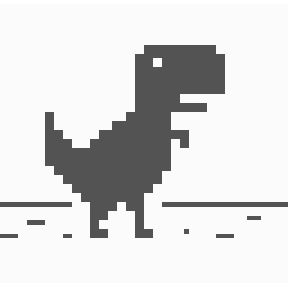
\includegraphics[width=1\textwidth]{files/dino.png}
    \vfill
    {\Large\bfseries\me{}}\medskip\par
    {\large\institute{}}%\medskip\par    
    %{\small\today{}}\medskip\par
    %\mybookaddress{} (\href{\mybookgithub}{Github})
\end{titlepage}
%\restorepagecolor
\newpage
\pagestyle{empty}


% \begin{figure}[h]
%     \centering
%     \includegraphics[scale=0.1]{files/IMG_0785.jpeg}
%     \caption{Two of my angels. They are breeding and laying eggs.}\label{fig:angelfish}
%   \end{figure}
  


\renewcommand{\contentsname}{Contents and Summary}
\tableofcontents


\chapter{Preface}

\mainmatter
\part{Introduction}\label{part:intro}
\chapter{Meeting}

\begin{itemize}
    \item Meeting is \emph{mandatory} for all lab members and is in-person.
    \item We meet \emph{every Thursday from 2pm to 3pm}.  Typically, our meeting directly follows the Software Engineering seminar (Thurs from 1pm to 2pm).
    \item We meet in the main CS conference room (Room \#4201 Nguyen Engineering Building).
    \item If you need to attend remotely, you can join via Zoom \url{https://meet.roars.dev} but you need to inform me ahead of time.
\end{itemize}
\part{Writing}

Oral and written communication is critical to research and science. You can create the most powerful systems with ground breaking results, but none of this matters if you cannot communicate or \emph{``sell''} these to others. 

\chapter{Publications}

% Writing papers
% 



% Further, I would argue that for technical HCI research particularly—where we build and study novel interactive systems—writing and scholarship is one of the primary differentiators between raw engineering/innovation, which you might do at a startup or tech company, and academic research. If you simply want to focus on building and engineering but not on science and scholarship then one must carefully reflect on whether a PhD is an appropriate investment and career path.
% The problem: writing is hard. It requires practice, iteration, and time. And academic writing is different, unlike any prior writing you have likely experienced. Even those first-year PhD students who are gifted writers or who have explicitly focused on developing their writing ability struggle with the transition to academic writing. I’ve written over 120+ scientific publications but I still consistently work on, study, and try to improve my academic writing.
% The opportunity: writing can be a huge differentiator in your career. It can improve your efficiency by reducing rejection rates and amplify your impact by making the results of your research interesting and understandable. You need to study great academic writing (and writers) and actively work on improving your skills. It will take time to hone your academic voice. Like any craft, it takes serious investment and practice. But it is worth it.
% Writing also has important intellectual benefits: it forces you to think deeply about your work, carefully articulate and contextualize differences with prior research, find gaps in your thinking or study design, and even has generative effects—you will think of new research ideas as you write (yay!).

% Figure. A metaphorical illustration of the generative effects of writing: writing forces your brain into thinking deeply
%  about a subject and unlocks new thoughts and possibilities. Source: David Perell. 

\section{Where do we publish?}

We aim to submit our work to the highest quality, most prestigious---``tier 1''venues but also the best fit for a specific project. 
Such top venues (generally) provides top peer review, a strong community of researchers, and if our work is accepted, provides visibility, credibility, and the opportunity for the most impact. 

\paragraph{Conferences}
Typically we aim for conferences considered by CSRankings, CSPicks (which includes CSRankings and CORE conferences) and other well-known ones in SE and PL. Depending on the topics of the work, we may also consider other venues.  For example, recently we also publish in Logics and AI/ML venues.

\begin{itemize}
\item SE venues: ICSE, FSE, ASE, and ISSTA. 
\item PL venues: POPL, PLDI, OOPSLA.  We have never published at POPL but it is a good venue for more theoretical work.
\item Logics venues: CAV and TACAS.
\item AI/ML venues: NeurIPS, ICML, ICLR, AAAI.
\end{itemize}

\paragraph{Journals}
Journals are not the main publication venue in most CS fields. However, we sometimes submit extended versions of our conference papers to top SE journals such as TSE and TOSEM.

\section{How to write research papers}
% There are three common writing applications for HCI publications: Google Docs, Microsoft Word, and Overleaf (LaTeX)—each have their merits. Overleaf has become the primary scientific authoring tool in our lab but Google Docs also plays a role in offering a lightweight space to collaboratively brainstorm ideas, outline sections, and potentially even drafting early sections; however, it is not an appropriate tool for actually writing submittable papers.
% Here is a document capturing LaTeX and TAPs tips started by PhD student, Chu Li.   
% To use Overleaf for an ACM submission, begin with the ACM Overleaf template. See ACM’s Overleaf page and Word webpage. Please make sure you use your cs.uw.edu account as the Allen School pays for a premium Overleaf subscription (and this gives us features like track changes, etc.)

\begin{itemize}
\item Always use LaTeX for writing papers. Do not use Word or Google Docs.
\item The paper should \emph{tell a story}. Humans are storytellers and story receivers.
  \item Be concise. Use the fewest words to communicate effectively.  For example, change ``In order to'' to just ``To'': that's 2/3rds cost savings for the same information.
   \item Avoid passive tense
   \item Know the difference between \emph{Such as} and \emph{like}
   \item Avoid long paragraphs
   \item Spell out numbers less than 10 (/three/ steps instead of /3/ steps).
   \item New paragraph for new thought/idea. Sentences in the same paragraph should be connected.
  %\item Use `~\cite{..}` and `~\ref{...}`: this ensures that the reference and figure numbers are not separated by a line break.
  %\item Use \code{\autoref} for figures, tables, sections, equations, etc.  This will automatically add the correct prefix (e.g., "Fig.", "Table", "Section", "Eq.") to the reference. E.g., `In~\autoref{fig:ex}, ...` gives `In Fig. 1, ...`
  % \item Use Eq. X instead of Equation X

% ### Miscs
% - Prefer high-level description than technical one
%   - People will not be interested in reading the rest if they can't understand (or get excited about) Intro
%   - Start technical sections with something high level, e.g., an overview picture or algorithm.  Don't go directly into formulae and theorems.  
%   - Before (or after) presenting some technical things (e.g., a theorem), explain why it is needed or useful.
% - Think of a presentation as an introduction to a paper (i.e., after seeing the slides, people will want to read the paper); and think of the paper as an introduction to the work/code (i.e.., after reading the paper, people will want to use your work/code).

\end{itemize}


% Interaction design is a largely visual discipline. So too then are HCI papers. We need to craft and tell visual stories. Here's a set of exemplary figures curated by the Makeability Lab to help you study and create the best figures for your papers!
% Scientific writing is rhetoric: your paper is an argument. What is new? What is different? Why do these differences matter? Notably, all of these statements can only be addressed comparatively by citing literature.

% Write rhythmically—draw your reader in with differently punctuated phrasings. But aim for concision.
% Do not use idioms (“on the other hand”) or cliches (“machine learning is not rocket science”)
% In prose, you should almost never have two sig figs after the decimal. Save such things for our tables (if even necessary there). Most of the time, two sig figs is overkill.

% My professional authorial name is Jon E. Froehlich. I should generally be last author on our papers together unless otherwise discussed.
% Related work is, in itself, plural. You should not say “Related Works.” Similarly, do not say “prior works” but rather “prior work.”
% Italicize all Latin abbreviations and words such as e.g., i.e., etc., et al., ad hoc, in situ
% All section and subsection headers must be followed by a strong topic sentence. No empty section/subsection headers with no prose.
% Numbers reported in prose should use one-sig fig (e.g., report 5.2 rather than 5.21). Two-sig figs is OK for tables and charts, as relevant.
% Italicize the first mention of a system. “In this paper, we introduce GazePointAR” in the Intro and first content section of the paper. Also italicize first mention of other systems (e.g., YOLOv8, Microsoft HoloLens 2)
\subsubsection{Writing Introductions}
The Introduction is the most important part of any paper. It must both excite your reader and provide a high-level view of your entire paper. Indeed, by the end of the Intro, your reader should want to read more but also have sufficient understanding about the key takeaways that if they stopped, they would ``largely get it.'' 

The intro has 5-6 paragraphs:
%And remember, your text alone is insufficient (even for the most gifted writers amongst us); your prose should be complemented by an amazing Figure 1 (see our “How to Figures” guide). 
% So, what are these 5-6 paragraphs?
% Para 1: Motivation and problem statement. Start with a compelling hook (a quote can work well, but don’t force it—here’s a lovely example from Chheda-Kothary et al.) then clearly begin defining and scoping your problem space.
% Para 2: Related work (RW) paragraph. What have others done to address said problem? What are some key benefits as well as drawbacks/gaps with past solutions? Frame limitations to help bolster offerings from the approach you provide in Para 3.
% Para 3: Our solution para. What are we doing to address said problem? What are key differentiating methods/benefits of our approach? As a writing crutch, think about starting this para with “In this paper, we introduce…” or “In this work, we examine…” (later, you might remove the “In this paper” part but good to keep for an initial draft.
% Para 4: Evaluation/validation para. How did you evaluate your solution? Explain the method, data collected, and analysis techniques. Use appropriate citations (e.g., generally we use well-vetted analysis techniques from the literature rather than pursuing something ad hoc, so cite that!)
% Para 5: Findings para. What are the key findings and takeaways? How do these findings advance the literature and what is currently known? Note: to make claims about advancements, you will inherently need to cite prior work. 
% Para 6: Summary of contributions.
% Now, of course, there are variations to any formula—so, appreciate this as a loose guide. For example, one common variation is to combine Para 1 and Para 2 so that your motivation para also introduces key RW and key limitations therein so that you can introduce your solution in Para2—this results in a five paragraph Intro rather than six. Similarly, you could imagine condensing Para 4 and 5 into one (the approach and the findings together).
% Moreover, this structure is more befitting of an HCI systems paper that introduces a specific solution to a problem. However, let’s imagine a different type of HCI paper—a formative inquiry or qualitative study paper. The formula (read: required paras) does change but not much:
% Para 1: Motivation and problem statement. Stays the same
% Para 2: RW para. Stays the same
% Para 3: Largely the same but introduce the key topical focus of the study and key research questions. “In this paper, we examine <some phenomenon>. Our research questions are threefold: RQ1: <write>, RQ2: <write>, and RQ3: <write>”
% Para 4: largely the same but now pivot to writing about how to address those RQs. “To address the above RQs, we conducted a three-part, semi-structured interview with 12 participants. <expand.>”
% Para 5: Findings para. Stays the same
% Para 6: Summary of contributions. Stays the same.
% Regardless, if you nail the above six things, you will have a strong Introduction.
% Also remember: each paragraph is only 4-6 sentences. Write concisely. This takes discipline and iteration. Your first draft will not be a perfect distillation of your arguments and key points; so, don’t worry about length until later drafts. For the initial drafts, focus on capturing the key arguments and points.
% Writing Discussions
% The key argument and differentiation for your paper is largely expressed through the Introduction, the Related Work section, and Discussion. These are the core argumentative sections; they are also all the most challenging to write. 🧠🤯 You must clearly situate and differentiate your work in the literature and emphasize why those differences matter. 
% The Discussion, in particular, is an opportunity to reflect on primary (and surprising) findings and situate them in the literature (think of phrases like “Our findings reaffirm those by Johnson et al. and Li et al. by…” or “In contrast to Smith et al., we found”). While Discussion sections also vary by paper type (e.g., Systems HCI paper vs. a qualitative study paper), they all generally:
% Restate and situate key contributions in literature (I often like to start Discussion sections with a summary of key findings situated in literature)
% Enumerate key limitations
% Highlight opportunities for future work
% If you included specific research questions (RQs) in your paper, it’s often useful to organize some Discussion subsections around those (e.g., see Arnavi’s Best Paper from ASSETS’24).
% Another way to organize your Discussion is around questions (as sub-headers). This is a fun and compelling writing device that helps draw your readers in and helps you (as a writer) organize your thoughts. Note: I don’t think you can do this for all your papers but it’s fun to consider. See:
% Lee et al., CookAR, UIST’24
% Hara et al., Tohme, UIST’14
% Here are some recommended Discussion sections from our lab:
% Study papers:
% Li et al., “I never realized sidewalks were a big deal”: A Case Study of a Community-Driven Sidewalk Audit Using Project Sidewalk, CHI’24
% McDonnell et al., Social, Environmental, and Technical: Factors at Play in the Current Use and Future Design of Small-Group Captioning, CSCW’21 Honorable Mention
% Saha et al., Urban Accessibility as a Socio-Political Problem: A MultiStakeholder Analysis, CSCW’20
% Jain et al., Autoethnography of a Hard of Hearing Traveler, ASSETS’19 Honorable Mention
% Jain et al., Towards Accessible Conversations in a Mobile Context for People who are Deaf and Hard of Hearing, ASSETS’18
% Mauriello et al., Understanding the Role of Thermography in Energy Auditing:
% Current Practices and the Potential for Automated Solutions, CHI’15
% HCI Systems Papers
% Froehlich et al., StreetViewAI: Making Street View Accessible Using Context-Aware Multimodal AI, UIST’25
% Lee et al., CookAR: Affordance Augmentations in Wearable AR to Support Kitchen Tool Interactions for People with Low Vision, UIST’24 Best Inclusion Award
% Saha et al., Project Sidewalk: A Web-based Crowdsourcing Tool for Collecting Sidewalk Accessibility Data at Scale, CHI’19 Best Paper
% Kang et al., SharedPhys: Live Physiological Sensing, Whole-Body Interaction, and Large-Screen Visualizations to Support Shared Inquiry Experiences, IDC’16
% Resources on paper writing
% Writing papers by Professor Eric Gilbert
% Writing papers guide by Professor Sean Munson
% How to write better discussions by Professor Daniel Buschek
% Five tweets of excellent writing tips by Professor Rodrigues
% How to write clear and concise sentences by Professor Huang
% Receiving feedback on writing by Dr. Karen Rosenberg, former Director of the Writing & Communication Center at the Bothell Campus
% TODO: need more on writing process. 
% Include different types of research contributions. Include different types of papers that can serve as templates
% Emphasize how iteration and practice is crucial. Give yourself time to write, rewrite x 10, and succeed.
% Sandy Kaplan and writing services within Allen School
% Often, junior students approach writing as they would a term paper in ugrad—it is left to the last moment. This approach will not succeed and does injustice to the underlying research. 
% Join a writing group: https://twitter.com/ThrivePhD/status/1433459109630824448?s=20. Provides structure and social support.
% Making Figure 1
% Need info on how to make accessible PDFs, etc.



\section{Authorship Inclusion and Ordering}
CS is a collaborative discipline. Most papers have multiple authors. However deciding who should be an author and the order of authorship can be challenging and a source of conflict. Below are some guidelines in our lab. 


\subsection{Inclusion}  


\begin{commentbox}
  As my student and co-authors, if you want to include some unobvious person as an co-author, you will need to discuss with me first before talking to other co-authors (e.g., collaborators). I can help determine if the person should be an author and help you discuss with others.
\end{commentbox}


If you have contributed meaningfully to a project, you should be an author. This includes:

\begin{itemize}
  \item People who contribute to the underlying research (e.g., design, implementation, evaluation, analysis). Typically these are students (or postdocs) who do the technical work.
  \item People who contribute to writing the paper (e.g., drafting sections, editing, providing feedback). These can be students, or collaborators, or PIs/advisors.
  \item People who are PI and fund the work, or direct advisor that allows the student to spend time on the project (this latter is more debatable but we are generous in our lab). Such people should also (or at least try to, e.g., participate in meetings) contribute to writing or discussions about the paper/work.  In any case, we always discuss authorship people ahead of time and ask if they want to be authors (some will say no).
\end{itemize}  



\begin{commentbox}[ACM's Criteria for Authorship]
Anyone listed as Author on an ACM submission must meet all the following criteria:
\begin{itemize}
\item They have made substantial intellectual contributions to some components of the original work described in the manuscript; and
\item They have participated in drafting and/or revision of the manuscript and
\item They are aware the manuscript has been submitted for publication; and
\item They agree to be held accountable for any issues relating to correctness or integrity of the work
\end{itemize}
\end{commentbox}


\subsection{Ordering}
\begin{itemize}
\item The first author is often the \emph{lead} student on a project, the last author is usually the PI or senior author, and the remaining authors are ordered based on contribution. 
\item Establish authorship order early in the paper writing process.  We do not want to have authorship disputes at the end of the process. Many conferences also require authorship order at submission time.
\end{itemize}



\chapter{Rebuttal}

\begin{itemize}
\item Start with a \emph{thank you note} to the reviewers for their time and feedback. Reviewing is a thankless job and reviewers often put in lots of time and effort to provide feedback.  Even if the reviews are harsh and you disagree, do it anyway. It can make them more receptive to your points.
\end{itemize}


% After submitting a paper and receiving reviews, HCI publication venues typically have two different processes for authorial responses (assuming the paper is not outright accepted): (1) revise and resubmit, which has been adopted by CHI and CSCW; (2) or a rebuttal process like at UIST and ASSETS.
% Writing rebuttals is hard: you are often space limited (to 5k characters) and must convincingly rebut reviewer criticism in hopes of changing minds. Plus, it is an emotional experience to read criticisms of your work, even if constructive. Remember, research is hard; this is a process. Your work is strong and strong work eventually finds a home. You can do this! 🚀
% To help guide you in writing, please see these resources:
% Attributes of a Strong Rebuttal and Things to Avoid, Jon E. Froehlich
% Jeff’s Rebuttal Guide, Jeff Bigham
% My Rebuttal-Writing Process for HCI Venues, Merrie Ringel Morris
% Technical Paper Rebuttals Aren’t Just for “Factual Errors”, Aaron Hertzmann
% For process, the best advice I can give is to:
% First analyze and synthesize your reviews. My students often use a spreadsheet or Google Doc to, essentially, generate an affinity diagram, which extracts and thematically groups primary criticisms.
% Second, write a draft rebuttal and iterate, iterate, iterate. Seek feedback from trusted colleagues. Iterate gain.
% Third and finally, be concrete and concise. See Attributes of a Strong Rebuttal referenced above.
% Finally, we have a collection of reviews and rebuttals from past papers (shared with permission). Please request access if you’d like to see them. Note: do not share these reviews or rebuttals as they are confidential.
% You might also benefit from the Writing Reviews section of our handbook.

% Preparing and giving talks
% “Tell someone a fact and you reach their minds; give them a story and you touch their souls.”
% - A Hasidic Proverb
% When you give a talk, you not only have an opportunity to demonstrate the strength and impact of your research but also your ability to organize and clearly articulate thoughts, to control and confidently adapt to an audience, and to tell a meaningful story. Like writing, giving a good talk takes serious preparation and rehearsal. But it’s worth it. In academia, there is a popular adage “every talk is a job talk.” I have found this to be true.
% In my group, I have long-emphasized that you can give an amazing, thought-provoking talk without slides but not the other way around—think Martin Luther King Jr.’s I Have a Dream speech, Amanda Gorman’s inauguration poem, or Abraham Lincoln’s Gettysburg Address. None had slides! The slides do not make your talk, you do. 
% Still, in HCI/d fields, well-designed slides are important, necessary, and reflect your aptitude and understanding of graphic design and visual communication. Slides are also necessary to properly capture our interaction design research! High-quality imagery and videos help highlight your incredible user interfaces and built artifacts. 
% One type of long-form, summative presentation is your “job talk”, which we cover in the Academic Job Talk section.
% Conference Talk Tips/Tricks
% Talks are unique mediums that are completely separate/independent from communicating science via a written publication. Do not treat them the same way! Do not formulate your oral communication with the same phrasing as your written communication (they are different!)
% You have to EARN your audience attention and then WORK to keep it throughout the talk
% Start with an undeniable hook that DRAWS your viewer in
% Leverage the unique multimodality of a talk: use your VOICE, use VISUALS, use VIDEOS, and use textual ANNOTATIONS
% If you say more than a single sentence without a backing written point or visual augmentation, you will begin to LOSE your audience. Thus, substantiate and complement your voice with the unique offerings of a modern presentation: images, videos, text
% On-screen text is critical but never write full sentences; use punchy text points
% Never use figures/images directly copy/pasted from your paper figures. Talks are a completely separate beast that requires a different type of visual communication. For example, observe how I introduce this rather complex graph slowly, introducing key elements first (and the skeleton for the graph) before animating in results and stepping my audience through key takeaways. Also note my :haircut: . :rolling_on_the_floor_laughing: 
% Your audience will hardly remember ANYTHING (want proof: think back to all of the conferences you have attended, what do you remember?). Thus, you need to really hammer in your key points and contributions. You can bring them up in the beginning of the talk and at the end. And again, be CREATIVE in how you get and sustain your audience attention
% Develop a commanding stage presence: do not read your slides, make eye contact, use gesticulation, modify the rhythm and cadence of your voice, draw your audience in with questions. Analyze your talk in terms of key beats---where will things be a bit more tedious for your audience? How can you followup that portion of the talk with something that again gets their attention?

% Resources
% TODO: resources for preparing good talks
% TODO: let’s list some of the best academic talks we’ve seen. 
% TODO: Here’s an old Dropbox folder of resources that I made. I need to go through this
% Writing Reviews
% In our field, our scientific papers are submitted to venues like CHI, UIST, ASSETS, and beyond and then undergo “dual-anonymous” (or “double-masked”) peer review. This means that both the paper is anonymous—we do not put our titles or affiliations on the paper for review—and that we do not know the identity of our reviewers.
% While review criteria can differ depending on field and publication venue, the primary criterion for judging a paper at CHI is “Does this submission provide a strong research contribution to the field of HCI?” This, of course, is not always so easy to determine and requires expertise in the field and an understanding of “strong”. For CHI’24, they’ve broken down review criteria into primary categories, including:
% Originality: what new ideas or approaches are introduced? We want to emphasize that an acceptable paper must make a clear contribution to Human-Computer Interaction;
% Significance: evaluate the paper's contribution to HCI and the benefit that others can gain from the contribution: why do the contribution and benefit matter?
% Research quality: how confidently can researchers and practitioners use the results?
% Previous work: is prior work adequately reviewed?
% Presentation clarity: how well is the paper framed and is the argument clear throughout the paper?
% Like anything, writing reviews takes time, effort, and iteration. You will get better with practice. There are also courses and online resources such as Professor Lennart E. Nacke’s short course previously offered at CHI How to Write and Review CHI Papers, which he has given since 2017 (see the course overview here, which also has some helpful advice).
% Example Reviews
% As a graduate student and junior scholar, I adopted a rigorous, critical eye for each review—carefully examining every section and sentence to determine quality and validity but with an overall philosophy of “this paper better prove to me it is worthy of acceptance.” I suppose, over time, I have softened my perspective: each paper and underlying system or study has flaws. The key is: does the paper advance the literature in interesting/impactful ways despite those flaws? Notably, this is a relativist framing not an absolute one and contributions, then, must be deeply situated in the relevant literature (by the authors, ideally) to assess such things. Moreover, my overall tone has shifted from one of criticism to one of support: how can I help the authors improve their work and correct underlying flaws?
% And perhaps my most important tenet: write a review like you would want received for your own paper. 😊
% Since my students have asked, I have provided some example reviews that I wrote 7+ years ago to help them better understand how I approach reviewing and structure my reviews (link). This is a private, curated set of reviews. Importantly, these example reviews are for my students only and not to be shared (students, please do not download them locally but view them in your browser). Even though much time has passed, revealing my identity for these reviews would break the principle of “double-anonymous” reviewing and, perhaps, cause emotional hardship or embarrassment for me or others.
% I am also happy to supply reviews we have received for any of our previous papers—assuming I still have them (sometimes, it is best to let them float away with time). Indeed, we provide some examples in the Writing Rebuttals subsection of this handbook.
% Resources
% Guide to Reviewing Papers, CHI’24
% An Unofficial Guide to Seven Stages of Reviewing for CHI, Neha Kumar, Sep 2020
% ACL’23 Peer Review Policies
% How to Become Good at Peer Review: A Guide for Young Scientists, Jennifer Raff, Dec 2023
% Making research videos
% Creating videos of your research is both a norm and expectation in HCI, particularly for UIST-style innovation or system work. While time consuming, creating a strong video to highlight your work can draw broad interest. Think about this: magnitudes more people will view your videos than ever read your papers. And the cost of preparing a strong video is amortized as you’ll be able to use video clips in your talk, on the Makeability Lab website, and more. So, we should aim to make videos for every project in our group! 📽
% This “Makeability Lab How to Videos” guide includes some exemplary videos curated by our lab as well as some guiding principles on making a good video.
% Here are some example videos from our group:
% ProtoSound video, CHI’22
% ARMath video, CHI’20
% Ondulé video, UIST’19
% ProtypAR video, IDC’19
% Project Sidewalk video, CHI’19 
% TouchCam video, IMWUT’17
% MakerWear video, CHI’16
% SharedPhys video, IDC’16
% BodyVis video, CHI’15
% Uploading and sharing videos
% As a lab, we decided in 2024 that our default option was to upload videos under the Makeability Lab YouTube account to create uniformity and maximize visibility; however, you are still welcome to instead upload your video to a personal account and we can link it with the Makeability Lab playlist.
% Note: we have tried other video hosting services in the past but they do not seem to draw as large of audiences (e.g., Vimeo).
% Intro sequence
% Movie studios famously use intro sequences for branding and visibility. Research labs do this too (e.g,. see example from Chris Harrison’s Future Interfaces Group). At UMD, some high school students and I collectively made the “HCIL Hackerspace” intro sequence in Adobe After Effects (see example); however, we never made one for the Makeability Lab (though I long wanted to!).
% Now, at UW, we finally have our intro sequence creating programmatically using p5.js and a custom reverse explosion animation (see p5.js program). My vision is to create an “infinite” number of these intro sequences based on this program (with different start locations, easing functions, and other animations). For now, I’ve exported one sequence and created three different videos:
% Makeability Lab Intro Sequence (2 secs)
% Makeability Lab Intro Sequence (5 secs)
% Makeability Lab Intro Sequence with DUB and CSE Logos (4.5 secs)
% Adding captions
% Creating accessible videos is important and a key ethic of our lab. It is best to not burn in your captions but rather to generate .srt or .vtt files that can be uploaded to YouTube or other services (.vtt files can also be associated with videos in PowerPoint to be able to selectively turn on/off captions). Our group recommends three captioning approaches:
% Adobe Premiere has built-in captioning tools, including automatic speech-to-text recognition
% If you don’t have access to Premiere, we suggest Happyscribe and Flixier
% Preparing and presenting posters

% Figure. An example research poster fair (at the Transportation Research Board conference in Washington DC). How will you make your research poster stand out? What will make someone stop at your poster to learn more?
% With a research poster, you have roughly 36”x60” to capture your viewer’s attention and communicate your research. My view is that the research poster is an advertisement for your paper, an advertisement for you (yes, you! And the team!), and should be designed as a visual aid complement to you standing there and communicating your research. Some tips:
% Make the title big, bold, attractive. Consider asking a question. The title should be readable from 15-30 feet away.
% Use visuals to communicate your story complemented by very little text.
% If you must use text, avoid prose. Use bullets.
% Remember, your poster will often be in a hall with ~100-200 other posters. How will you grab your viewers attention? As a passerby walks by, what will make them stop? If you have a wall of text, they will just move right along. See figure above.
% Good and Bad Poster Designs
% Figure. A famous poster redesign by Michigan State University doctoral student Mike Morrison. Image from NPR. Notice how it draws you in from afar. And then once you walk close, you can read a bullet-pointed overview augmented by visuals.
% Here is but a small selection of some of my favorite posters from the Makeability Lab:



% BodyVis poster by UMD MS student Leyla Norooz (great use of graphics & colors; however, fonts are too thin and insufficient contrast with text colors and background)
% Ondule poster by UW PhD student Liang He (again, great use of graphics, clearly communicates research, maybe a bit visually busy)
% Social Fabric Fitness poster by Jon E. Froehlich (in retrospect, too much text; should have eliminated 80% of the text and bullet pointed but the poster does draw you in with the graphic and question)



% In contrast, here is a poorly designed research poster: text heavy, no clear reading direction, boring.

% Figure. A poorly designed poster example (from Better Posters)


% What tools to use?
% I tend to make my posters in PowerPoint (go into the Design tab and set the Slide Size to Custom Slide Size of whatever your dimensions are—for example, 34” x 56”). Note that PowerPoint limits their max slide size to 56” x 56”.
% Others use Adobe Illustrator (e.g., FuzzPrint), Photoshop (e.g., TacTILE), or Figma (e.g., BusStopCV, Sidewalk Equity)
% Where to print a poster?
% In the Allen School, we are fortunate to have a poster printer! You can learn more about using it here. This is useful for Affiliates Day and other on-campus events. For a conference that requires travel, you can print a poster in the Allen School and travel with it using a carrying tube. Or, you can print the poster at your destination (if you know a poster printer is available).
% Resources
% A Graphic Design Revolution for Scientific Conference Posters, Forbes, 2019; Eva Amsen
% To Save the Science Poster, Researchers Want to Kill it And Start Over, NPR, 2019; Nell Greenfieldboyce
% The Better Posters Gallery, which is part of the Better Posters blog by Zen Faulkes
% Better Posters Blog, by Zen Faulkes

\chapter{Writing Styles and File Organization}

Every one has their own way of organizing files and writing papers. Below is my approach that has worked well for me over the years. If you're my student and write papers with me, I expect you follow this approach so that I can easily find things.  

However, if we collaborate with others, we can adapt how we write and organize files as needed. Typically, the main group lead will decide how to organize things and the rest of us will follow their lead.  For example, if we lead a paper, then we will follow my approach below.  But if we collaborate on a paper led by others, then we will follow their approach.


\section{File Organization}\label{sec:file-organization}


\begin{enumerate}
\item Create a separate Github Repo for each \emph{project}.
\begin{itemize}
  \item The reason is that we will likely write multiple papers for the same project (e.g., conference papers, journal papers, workshop papers, etc). Having a single repo per project makes it easier to manage and find things.
  \item Name the repo \code{paper\_projectname}, e.g., `\code{paper\_gentree}` where \code{gentree} is the name of the work.
\end{itemize}
\item Within the repo, create a separate directory (folder) for each \emph{paper}.
  \begin{itemize}
    \item Name the directory based on the venue and year, e.g., \code{icse2025} for a paper submitted to ICSE 2025.
  \end{itemize}
\item Within the paper directory, I use \emph{very few} files (e.g., the entire paper in a single TeX file).   Typically, I have the following:
  
\begin{enumerate}
  \item \code{paper.tex}: a \emph{single} \code{TeX} file for the entire paper. 
  \begin{itemize}
    \item Others might prefer using multiple files / directories (e.g., \code{intro.tex}, \code{eval.tex}, \code{sections/related.tex}. But I find it easier to just use a single file because I can easily search and replace for things and I don't have to switch between files.
  \item Even when sharing or collaborating with others, in which conflict edits can arise, a single file still works well because Git is pretty good at resolving conflict issues. Note that I do have conflicts with this approach, but they also happen with multiple files.
      \end{itemize}
  \item \code{paper.bib}: A single \code{bib} file for bibliography references.
      \begin{itemize}
        \item I prefer a single bib file because it is easier to manage and search for references.  Others might prefer multiple bib files (e.g., \code{refs1.bib}, \code{refs2.bib} for different sections).
        \item My collaborators sometimes put in their own bib files.
      \end{itemize}
  \item \code{figures/}: A directory (folder) containing all figures for the paper.

\end{enumerate}


\end{enumerate}
  

% ## After submission

% After submitting a paper, I save a copy of the submitted pdf file and create a tag for the latest commit to keep a history of that submission.
% 1. Save the submitted pdf file as `VenueYearX.pdf`, where `X` is submit for the original submission version, `final` for final (camera-ready) version and `rI` for the `ith` revision for additional revisions between the original submission and final (e.g., for jounal).

%     ````
%     git add icse2021submit.pdf  
%     ````

% 2. Then create an annotated tag for the commit
%     ````
%     git tag -a icse2021submit -m "ICSE 2021 original submission" commit_hashid (optional)
%     git push origin icse2021submit
%     git show icse2020submit
%     ````

% ### After rebuttal

% After submitting a rebuttal, save a copy of the reviews and rebuttal as a plain `text` file

% ````
% git add pldi2023-reviews.txt
% git commit -am "reviews and rebuttal"
% ````







\chapter{Presentation}

\begin{itemize}
  \item \textbf{Title slide} with paper title, authors (highlight or underline the presenter's name), affiliations, conference or event name, date.
\item \textbf{Number your slides}.  This is useful when people want to ask questions (or give feedback) on specific slides (e.g., \emph{``on slide 10, you said ...''}).
\item \textbf{Every slide takes approximately 1 minutes}. Using this rule of thumb, you can estimate how many slides you need for your presentation.
\item \textbf{Avoid Technical Stuff}.  Avoid slides that are too technical (e.g., formulae, code snippets, algorithms, etc) unless absolutely necessary. \emph{Focus on motivation and high-level ideas}.
\end{itemize}


\chapter{Data and Code Management}
\section{Data Availability}
\begin{itemize}
\item We will \emph{always} make the data available. So make sure prototypes, tools, results, etc are avail on Github.
\item Github repo:
\begin{itemize}
\item \texttt{README.md}: include a description of the project, how to install and use the tool.
 \item For tools submitted to conferences, include scripts to generate the data and run the experiments.
\end{itemize}
\end{itemize}

\part{Miscs}

\chapter{Advice}

\section{Grab Opportunities Quickly} As you will see in research, opportunities come and go quickly. You might be quite stagnant for a while, and then suddenly an opportunity appears (e.g., a new idea, a new collaboration, a new funding source, a new place to submit papers, etc). You need to be ready to grab these opportunities quickly.  So be ready to jump on opportunities when they arise.

These opportunities might not be specific for you but for your research group or lab. So if you see something relevant, bring it up, e.g., post on our group Discord or email me/the group members directly.

\begin{commentbox}[Example]
    I was browsing Linkedin one day and saw a post about the NFM'26 submission, whose deadline was in two days. I quickly send emails to my students to see if they want to resubmit some of our previous work there. One student quickly agreed, and we quickly prepared a submission in two days.
  
\end{commentbox}  


\part{Classes}

\begin{itemize}
\item Independent Study
\begin{itemize}
    \item You need to be my student before you can register for independent study with me.  I.e., unless I officially advise you, you cannot register for independent study with me.
    \item You will typically get an A grade if you do the work satisfactorily. This is one of the reason why PhD students often get high GPAs, and also the reason why no one cares about your GPA after you got a PhD.
\end{itemize}
\item Dissertation/Thesis Credits
\begin{itemize}
    \item Register for CS 998 (Dissertation Proposal) for ..  
    \item Register for CS 999 (Dissertation) for ...
    \item If you perform satisfactorily in your research, you will get an \textbf{IP} (in progress) grade, which then converted to S (satisfactory) at the end of the semester when you advance to candidacy (for CS 998) or graduate (for CS 999).
    \item If you do not perform satisfactorily, I will talk to you directly. 
    \item If I cannot even reach you, I will give you an \textbf{NC} (no credit) grade. This can happen, e.g., in a case I said I would be willing to give the student a try but the student never contacted me during the semester or made any progress. 
\end{itemize}
\end{itemize}




\part{Reimbursement}



\part{Equipment and Resources}
\chapter{Connecting to Wifi and VPN}

\section{Connecting to VPN}
TBD


\chapter{Lab Servers}


% Makeability Lab Resources
% As lab PI, I want to provide you with the resources and equipment necessary to do your research, fulfill your potential, and be successful. If you need something, please ask. I will work with you on a solution.
% Communication
% We primarily use Slack and email for communication:
% Mailing me. If something is important and you want me to add it to my work queue (e.g., give feedback on a design mock, review a paper draft), please email me at jonf@cs.uw.edu. You can also ping me on the Makeability Lab Slack. It’s best to include a deadline so I can prioritize when to provide feedback. Please follow-up if you do not hear back. I don’t mind!
% Mailing lists. We have multiple Makeability Lab mailing lists. For current PhD students, I will often email announcements or forward opportunities to makeabilitylab-grad@cs.uw.edu. We also have a general makeabilitylab@cs.uw.edu that goes to all active students (high school, ugrad, grad) and makeabilitylab-alumni@cs.uw.edu.  
% Slack. For synchronous communication and more informal chats, we use Slack: https://makeabilitylab.slack.com. If you’re on the Project Sidewalk team, please join both the Makeability Lab Slack and the Project Sidewalk Slack: https://projectsidewalk.slack.com.
% Twitter. Our lab maintains two Twitter accounts: @makeabilitylab and @projsidewalk. Jon is at @jonfroehlich.
% Makeability Lab website. We post all projects and papers to the Makeability Lab website. When you join the lab, you should get added to the lab website.
% Lab Space
% The Allen School is privileged with lab space, which brings choice and opportunity. Ideally, to build rapport between us, we would all work in the same lab space. I realize, however, that preferences and needs differ. For example, some of us work with hardware, others do not.
% There are two hardware/fabrication lab spaces. You need to sign up for training to use this equipment. Email Alexander Lefort and sign up for the fablab mailing list.
% The Ubiquitous Computing Lab (Ubicomp Lab) in the Allen Center (CSE 605 & 615). I moved my office to CSE642 specifically to be close to the UbiComp Lab. My preference is that you use this as your primary lab space given its proximity to my office and the opportunity to intermix with UbiComp Lab students.
% The FabLab in the Gates Center (CSE2 G15)
% And two HCI lab spaces:
% The HCI Lab in the Allen Center (CSE 591)
% The HCI Lab in the Gates Center (CSE2 283)
% Lab Access
% To request lab access, send an email to cardkey@cs.washington.edu and CC me with the specific location (e.g., UbiComp Lab in CSE605) with a specific date range.
% HCI/UbiComp Lab Spaces
% The Ubicomp Lab (CSE 605)

% Figure. Pictures of the Ubicomp Lab workspace (CSE605) and neighboring fabrication space (CSE615). You can access CSE615 via CSE605.
% The UbiComp Lab (CSE 605) has 21 assigned seats for research assistants and a connected fab lab (CSE 615) with 3D printers (e.g, Stratasys F370, F120, Form 3, and Ultimaker 3), laser cutters (e.g., Glowforge), a reflow oven (LPKF ProtoFlow S), and soldering stations. 
% To request a seat, please email me so I can work with Shwetak on lab assignments (the seat chart is here).
% To request keycard access to the fab lab side (CSE615), please email cardkey@cs.washington.edu and CC me
% The FabLab (CSE2 G15)

% Figure. Pictures of the FabLab in CSE2 (G15). You need training to use these spaces and some equipment requires additional training.
% The FabLab (CSE2 G15) is not intended as a fulltime workspace but rather a place to drop in for specialized fabrication projects. Besides three desktop 3D printers (2 Ultimaker 3 extended and 1 Form 3) and a laser cutter (Glowforge), this lab offers more advanced equipment options. To name a few (see figure below): knitting machine Shima Seiki SWG091N2, Stratasys-FDM 3D printers F170/f120, Desktop Metal 3D Studio printer, Stratasys Objet 30 polyjet 3D printer, Trotec Speedy 300 laser cutter,  LPKF Protolaser S4 PCB laser cutter, ShopBot PRS-Alpha CNC router, Drill Press Powermatic PM2800B, and Tablesaw Sawstop JSS Pro. Please check the full list of equipment on the official website of FabLab. To use this equipment, please reach out to the lab manager Alexander Lefort (aalefort@cs.washington.edu) for training first. 

% Figure. Pictures of the FabLab equipment in CSE2 (G15). 
% Allen Center HCI Lab (CSE 591)
% Figure. A picture of the Allen Center HCI Lab (CSE591) with ideation spaces and a few desks for working..
% The Allen Center HCI Lab (CSE 591) provides a casual and collaborative ideation space with a whiteboard, projection screen, and couches as well as eight desks for graduate students and postdocs. Currently, the lab is mostly inhabited by Professor Reinecke and Fogarty’s students.
% Gates Center HCI Lab (CSE2 283)

% Figure. A picture of the Gates Center HCI Lab (CSE2 283) with a hardware workshop, ideation spaces, and a few desks for working.
% The Gates Center HCI Lab (CSE2 283) provides a casual and collaborative ideation space with a large whiteboard, a mini-workshop for tinkering on hardware projects, and couches as well as six desks for graduate students. Currently, the lab is mostly inhabited by Professor Mankoff’s students.


\chapter{Lab Website and Other Online Resources}

\begin{itemize}
\item Our main Roars lab website is at \url{https://roars.dev/}.  It is in plain HTML. All code is open source and available on GitHub (\url{https://code.roars.dev}).
\end{itemize}
% Our lab website is at https://makeabilitylab.cs.washington.edu/ and is built in Django (Python). All code is open source and available on GitHub (link). We currently have over 100 open issues. If you like web development and/or have Django experience, we would greatly appreciate your help. 🙏
% If you are a grad student or research scientist in our lab, you should:
% Make project pages
% Add in news
% Add your publications
% You can use the gradmin account (Slack us for the password). Xia Su is currently our lab website manager. He can help you!
% Lab Photos
% Our lab history and time together is captured (in part) by our collection of photos and videos stored here (this is a private link for Makeability Lab members only).
% Lab GitHub
% We use GitHub religiously for hosting and coordinating our research projects. Your code can begin in a private repo but should be released on the Makeability Lab organization, when possible, when your research is published. One exception is Project Sidewalk, which exists as its own GitHub organization.
% Generally, we aim to support open science, which means releasing our code and datasets for scientific replicability and to enable future research. README.md should have clear instructions, compelling visuals, and descriptions on how to replicate the scientific work. Please also include a citation (e.g., if you use our code, datasets, or ideas in our paper, please cite us as <include bibtex>). Some good model repos are:
% CookAR
% RampNet
% Kind reminder: you should never write research code without continuously backing it up (ideally, using a version control system like Git) but, in the worst case, Dropbox, GDrive, Box, iCloud, etc.
% Lab Logos
% Here are links to logos for the Makeability Lab, the Allen School and UW, and UW CREATE. The logos for Project Sidewalk are in the Project Sidewalk Design GitHub repo. Logos should be used on the first and last slide. Here are some ideas/templates.

\chapter{Useful University Resources}

\begin{itemize}
  \item \textbf{Printing Posters}: \url{https://library.gmu.edu/poster-request}.  Request 3 days in advance, pick up at Fenwick Library, completely free for GMU faculty and students.  \emph{Excellent service and yet no one seems to know about it!}
  \item 
\end{itemize}  

% Accessing CSE Linux Servers
% The Makeability Lab website, Project Sidewalk, and even your academic website runs on CSE Linux servers. It’s fastest and easiest to setup an SSH key to quickly SSH into these servers.
% Mac/Linux
% On Mac or Linux, open up the terminal. Run:
% > ssh-keygen
% Hit <Enter> to accept the defaults (no passphrase needed). The key will be saved in ~/.ssh/id_rsa and the public key in ~/.ssh/id_rsa.pub.
% Then, again in terminal, run:
% > ssh-copy-id user@host
% So, for example, I would run
% > ssh-copy-id jonf@recycle.cs.washington.edu
% Here, you’ll be asked to login for the final time with your password. Once this completes, you should be able to do this:
% > ssh jonf@recycle.cs.washington.edu
% And it will succeed without having to enter a password.
% Windows
% On Windows, open up Windows Powershell and type:
% > ssh-keygen
% Hit <Enter> to accept the defaults (no passphrase needed). The key will be saved in $env:USERPROFILE/.ssh/id_rsa and the public key in $env:USERPROFILE
% /.ssh/id_rsa.pub.
% Unlike on Mac/Linux, the command ssh-copy-id does not exist, so to move your key onto the server, you need to do something else:
% > type $env:USERPROFILE\.ssh\id_rsa.pub | ssh {IP-ADDRESS-OR-FQDN} "cat >> .ssh/authorized_keys"
% So, in our case, we would type:
% > type $env:USERPROFILE\.ssh\id_rsa.pub | ssh recycle.cs.washington.edu "cat >> .ssh/authorized_keys"
% The server recycle.cs.washington.edu will ask you to login one last time with a password. Once you do that, you should be able to login without one.




\appendix
\chapter{LoRs}

\section{New Member}

Some quick steps for new faculty members to get started in the CS dept.

\begin{enumerate}
\item Know your G\#. You will need this for many things.
\item \textbf{Email}: GMU will setup your account and email automatically. Your initial email will be something like \code{tngu94}, but you could ask to change it to something else nicer like \code{tvn}.
\item \textbf{Webpage}: Email CEC IT (\url{mailto:cechelp@gmu.edu}) to setup an account on the CS home server so that your webpage \url{https://people.cs.gmu.edu/~username} can be created. 
\item \textbf{Office/Key}: 

% 0. Obtain from Deb Heckens (2-3200) a cost center for your startup fund. This is simply a
% 10-digit number that allows you to charge your expenses to.
% 1. Talk to Shea Svoboda to get a cse.unl.edu account. You should be able to get the
% account within a few minutes.
% 2. Talk to Shea Svoboda to get your computers setup. If you are buying new computers,
% please specify their configurations with Charles. Charles can get you cheap computers from
% D&amp;E (a contracted company).
% · Turn in your specifications to Deb Heckens (2-3200) so she can make the purchase order.
% · It takes a while (may be 14-20 days) before your computer arrives. So plan early.
% · Check to make sure that the ports in your office are activated. If not, then have Sally
% Hawkins (2-5001) put in a request for you. The activation process will take 3-4 days to a week.
% You may contact the Information Services (Mike Davidson, 2-5766 or 2-5785) directly after the
% request is put in.
% · Meanwhile, you can ask Charles to give you a temporary computer for your office or you
% can use the computers in Rooms 16 and 17 to check your e-mail.
% 3. To get a NCard ID, please go to the Nebraska Union (student union). They will take
% your picture and give you the card right there. No prior appointment necessary.
% · You can also get a free bus pass with you NCard ID. Sometimes, the buss pass is not
% available until a couple of days before the semester starts. To get the bus pass, go to the
% Information Center at the student union.
% · Get your NCard ID as soon as possible before doing anything else. Make things easier as
% you can use your NCard ID to get a parking permit, for example.
% 4. Furniture. If you do not have enough furniture in your office, please call John Lohmeyer
% (2-1187) of the Inventory Warehouse to setup an appointment with him so that you can visit the
% warehouse to secure some used furniture items. Usually, the Warehouse has an OPEN day
% every Wednesday. The used furniture items are free. But the delivery of those items to your
% office is not. So, you have to give them your cost center at the warehouse after selecting your
% furniture.
% · The delivery will take about 10 days. So, plan early. The person in charge of the delivery
% is Bob Gier (2-2678). After selecting your furniture and after a week of waiting, you may want
% to call Bob Gier to find out the current status of your furniture.
% · Note that the warehouse is over on the East Campus.
% · NEW PROCEDURE: Now, you have to call Bob Gier yourself. Actually, you have to ask
% Deb to FAX Bob Gier (2-7051) a requisition form with the description of your furniture items on
% it.
% 5. To get yourself on payroll and benefits, please check with Deb Heckens (2-3200) before
% going to the 501 Building for Human Resources.

% 6. If you want to hire some graduate students for your projects (from your startup), please
% go to Shelley Everette (2-7760) early to get the list of potential candidates. These candidates
% are ranked and reviewed by the faculty and they are the best of the student population.
% 7. To get miscellaneous items such as calendar, stationary, etc., go to Sally Hawkins (2-
% 5001). She will be able to give you those items or order them for you.
% 8. For nailing and installing bulletin boards in your office, please go to one of the student
% assistants at the CSE office. Usually, there will be one hired to help out with the office work.
% You may ask him/her for help. The CSE office does have a toolbox.
% 9. To get your semester started, make sure that you give Shelley Everette (2-7760) the list
% of textbooks you want to have for your classes. Do this as soon as possible.
% · To check whether the books are in, check with Shelley Everette (2-7760) or the bookstore
% (2-7300).
% 10. Obtain the keys to the building, department office, and your office from Sally Hawkins or
% Deb Heckens (2-3200).
% 11. Set up a pin number to use the photocopy machine in the mailroom from Shelley Everette
% (2-7760).
% 12. Set up your mailbox in the mailroom from Shelley Everette (2-7760) or Sally Hawkins (2-
% 5001).
% 13. The roster of your class will be in your mailbox a day or two before the semester starts. So
% don’t worry about it.
% 14. The TA of your class will be assigned to you probably a few days before the semester
% starts. So, don’t worry about it.
% 15. Set up your voice mail system as soon as possible. Call 2-3434 for help.
% · You will receive your voicemail information after 3-4 days, telling you how to setup your
% password, among other things.
% 16. Make sure that your mailbox has been installed to activate the message waiting lamp on
% your phone. If it has not, please go to Deb Heckens (2-3200) to have her set it up for you. It
% costs money. But the department will pay for it. You should not have to.
% 17. You have one month of free parking. You have to get that free parking permit from the
% Parking and Transit Service (2-1800).
% 18. Then to get your area-10A (Red) permit, you can get that from the same Parking and
% Transit Service office (2-1800) too.
% 19. To use the Campus Recreation Center, you need to get a membership. It is now about
% \$18/month for a faculty. It has an option that allows the fee to be deducted directly from your
% payroll. This center is well-equipped. Basketball, badminton, volleyball, ping-pong, running
% tracks, weights, exercise machines, etc. 2-3467.
% 20. If you have some research-related contract questions, please go to Suzan Lund (2-3171).
% She is Associate Director of the Sponsored Programs at UNL. This is only for research projects.
\end{enumerate}

\section{Asking}

\begin{itemize}
    \item If you want a letter from me, you should \textbf{ask} at least 2 weeks in advance (ideally a month).
    \begin{itemize}
        \item \textbf{DO NOT} put my name in the application system without explicitly asking me first.
    \end{itemize}

    \item If I don't know you well enough, I will let you know and advise you to find someone else. But if you insist, I will still write you a letter.
    \item You need to \textbf{waive your right} to view the letter. It is a confidential evaluation, and I will not write one if you insist on seeing what I write.
    \item You should provide me your CV and, if you'd like, your SOP, so I can determine whether I could complement some of the things you've said.
    \begin{itemize}
        \item Feel free to provide me with any other information that you think is relevant, e.g., your grades, projects, research experience, awards, etc. I might not use them if I don't think they are relevant, but they might help if I miss something.
    \end{itemize}
\end{itemize}

\section{Writing}

\begin{itemize}
    \item I \textbf{will not ask you to draft a letter} for me. My reputation is on the line, and I do not want a student (or AI) writing a letter on my behalf.
    \item I \textbf{do not write negative letters}, i.e., I don't say bad things about you (even if you're bad). However, if I don't know you well then a neutral, short, or generic letter will not help your case given the competitiveness.
    \item It takes me about \textbf{an hour} for a strong letter for someone I know well, and about 10 minutes for a letter for someone I don't know well.
    \item In all letters, at the end I will include a short paragraph about \textbf{an area you need to improve}, regardless of whether you're super strong or weak. But I will phrase it in such a way that the graduate study environment or a good advisor can help you overcome it. It makes the letter more complete and not just full of praise.
    \item I \textbf{do not customize} the letter for specific schools.
    \begin{itemize}
        \item You customize your SOP to explain why you want to apply to school \texttt{X} and work with professor \texttt{Y}. I do not need to explain why you want to go to school \texttt{X} or why you would be a good fit for professor \texttt{Y}. Note that if I know you and \texttt{Y} very well, then I might send a letter directly to \texttt{Y} to mention you.
    \end{itemize}
    \item My letter will have the university logo and my (digital) signature.
    \begin{itemize}
        \item However, I should note that when I read a LoR, I do not pay attention to whether it has a logo or signature.
    \end{itemize}
\end{itemize}

\section{Sending}

\begin{itemize}
    \item After you put my email into the application system, it will send me a request email with a unique URL to go to. It will also give me some deadline that is \emph{likely} not the same as yours---usually later.
    \begin{itemize}
        \item In some cases the systems don't even give me a deadline (various LoR request examples are shown in my \texttt{Demystify} book, e.g., Section 3.2.3: \href{https://github.com/dynaroars/phd-cs-us/}{https://github.com/dynaroars/phd-cs-us/}).
    \end{itemize}
    \item I \textbf{do not mind if the student is anxious and sends me multiple reminders}. I will likely not respond to them. But I am not bothered by reminders. Over-communication is better than under.
    \item Most systems simply ask me to upload the letter---though a few have short questions like comparing the applicant to undergrads or grad students. As an adcom reviewer, I don't really pay attention to these comparisons---only the letter matters.
    \item I usually send my letter (in PDF) in \textbf{batch mode}, e.g., I just sent out 10+ letters all at once and cleared my inbox of these requests.
    \begin{itemize}
        \item For each request, it took me less than 30 seconds to upload the PDF and hit \texttt{submit}. So do not worry that it is time-consuming or a burden; it's not.
    \end{itemize}
    \item After I send my batch, I'll let you know I just sent everything and ask if I missed any.
    \begin{itemize}
        \item I would appreciate if you share an online spreadsheet showing what schools you have asked me to write letters for so I know what to expect (and if I miss something).
    \end{itemize}
\end{itemize}

\section{Updating}

\begin{itemize}
    \item Let me know your progress and especially your outcomes, e.g., interviews, offers, and where you eventually go to. I'd love to hear these updates from you.  
    \item This is a common courtesy. Though I probably won't remember or expect you to do this.  However, if you do this and then years later reach out for another letter, I might not be able to help you.    
\end{itemize}
\chapter{Templates}


%\bibliographystyle{abbrv}
%\bibliography{demystify.bib}

\end{document}







----











# Building a machine for Neural Network Verification

We have just built a new machine **"PizzaBox"** for our research group.  Linhan and Hai built it on Oct 31st (Halloween) and it is up running since Nov 1.  The machine will be mainly used for our SE/PL research. In particular, we will use it for **neural network verification**, which is a bit different than an ML machine that focuses on training and therefore requires different hardware components and setup.

This machine is both cheaper than a machine with similar specs from Dell or Lenovo. It also runs a lot faster than computer servers available at GMU that we have access to.  We believe such customized computers are best for our purpose and hope that this post will be useful for others who are interested in building a similar machine.

## The Specs and Cost 

| Hardware | Details     | Cost | Notes |
|----------|-------------|------|-------|
| Motherboard| [ASUS Pro WS WRX80E-SAGE SE WiFi II AMD](https://www.amazon.com/gp/product/B0BZT9NF57/ref=ppx_yo_dt_b_asin_title_o05_s03?ie=UTF8&psc=1) | $1,070.52 | | 
| CPU      | AMD Ryzen™ Threadripper™ PRO 5975WX, 32-core, 64-Thread|  $2,749.98 |  from Microcenter
| GPU      | [GIGABYTE GeForce Nvidia 4090 RTX 24 GB VRAM](https://www.amazon.com/gp/product/B0BGP8FGNZ/ref=ppx_yo_dt_b_asin_title_o04_s00?ie=UTF8&th=1) |$1,699.99 | |
| RAM     | [Corsair Vengeance LPX 128GB](https://www.amazon.com/gp/product/B085WQXKM2/ref=ppx_yo_dt_b_asin_title_o05_s02?ie=UTF8&th=1) |$259.99 |
| HD  | [Western Digital BLACK 2TB SN850X NVMe](https://www.amazon.com/gp/product/B0B7CMZ3QH/ref=ppx_yo_dt_b_asin_title_o07_s00?ie=UTF8&th=1) |$119.99 | 
| PSU | [Corsair RM1000E](https://www.amazon.com/gp/product/B0BYQHWJXC/ref=ppx_yo_dt_b_asin_title_o05_s00?ie=UTF8&psc=1)|$179.99 | 
| Case | [CORSAIR 7000D AIRFLOW Full-Tower--WHITE](https://www.amazon.com/gp/product/B09444VWX2/ref=ppx_yo_dt_b_asin_title_o02_s00?ie=UTF8&th=1) | $244.99 | 
| Fan (CPU) | [Cooler Master](https://www.amazon.com/gp/product/B07H25DZ3M/ref=ppx_yo_dt_b_asin_title_o06_s00?ie=UTF8&psc=1) | 119.00 | 
| Fan (Case) | 4 x Noctua 140mm  | $23.95 | | 
|    |         |**$6,468.4**   |    |


The CPU and GPU are the two main components we need for our DNN verification. The other components are flexible.  For CPU, we go with the AMD Threadripper 32 cores (64 threads).  This is the 2nd, not top, of the line because the Threadripper 64 cores costs quite a bit and would require additional paperwork to purchase.  For GPU, we go with the current top of the line for gaming, the NVIDIA RTX 4090.  


## Timeline
- 9/11: order components
- 10/31: complete the build (1 day)

## Building It
> *Before you start*
> - make sure to discharge yourself before touching the parts.


- **Open the boxes!**
- **Install SSD, CPU, RAM:**
  - _It's often a good idea to install smaller parts onto the motherboard first._ Working in the chassis can be more challenging due to limited space.
    - **CPU:**
      - Our CPU (59775wx) uses an sWRX8 socket. The installation is a bit different from the other consumer CPUs we've seen, so it took us a while to read the manual and figure out how.
    - **SSD:**
      - Very typical NVMe SSD installation. We removed a cover from the motherboard to expose the M.2 slot, and installed the SSD in the M.2_1 slot (M.2_1 is usually directly connected to the CPU, which gives better performance).
    - **Install RAM:**
      - Nothing special about the RAM installation, either. The CPU & MB together have 8 RAM slots, each with a dedicated channel, so we used every other slot for better thermal performance. On some MBs, multiple slots might share a channel; when this happens, the MB's manual will tell you what to do.
- **Install MB:**
  - Now we can put the MB into the chassis. The chassis comes with extra standoffs and panels for ATX MBs, so we had to remove them before proceeding (because we're using an Extended-ATX, which is larger). Fit the I/O panel into the slot on the back of the chassis, and align the standoffs to the holes on the MB. Lastly, tighten the screws in an alternating pattern (so the force is evenly distributed).
- **Install PSU:**
  - Our MB was interesting; it has one MB power connector, two CPU power connectors, and one extra PCIe power connector (which is not common). The GPU uses one of the 12VHPWR connectors. We attached the cables to the PSU first, because it will be much harder to add power connectors once the PSU is in the chassis.
- **Install fans/airflow configuration:**
  - We used the conventional airflow configuration, front-to-back/top. The 140 mm fans by Noctua are really powerful yet quiet. When shopping for fans, we aimed for airflow, not air pressure, because we're not using an AIO cooler (AIO needs higher pressure to push the air through the radiators). Once we installed the fans, we routed the wires to the back of the MB, preparing for cable management.
- **Install CPU cooler:**
  - Our cooler comes with thermal paste pre-applied, so all we did was put it on the CPU and tighten the screws in an alternating pattern. This fancy cooler has a 4-pin fan connector and another SATA power connector for RGB (which none of us care about).
- **Install GPU:**
  - To install the GPU, we had to take off the PCIe slot covers. Our GPU uses two slots, so we took off two of the covers, and then we just snapped the GPU into the 1st PCIe slot. Because the 4090 is so heavy, we had to order an additional GPU supporting bracket, or the MB would be at risk.
- **Connecting cables/cable management:**
  - The last step is to connect the cables. It's simple but kind of tedious. The only potentially challenging part is connecting the system panel connectors (power button, restart button, etc.). Cable management is optional but recommended; it requires patience and some skill. 
- **Test build/install OS:**
  - After connecting everything, we pluged in the power cord and gave the system a test drive. The hardware works as expected and everything was detected by the MB. So, we continued to install the OS. However, this didn't work as well as we expected. The system boots into the installation media with no issue, but as soon as we start the installation, the keyboard stops working. After spending a couple of hours looking for a solution online, we found out that disabling SR-IOV does the trick. Strange. [link](https://www.overclock.net/threads/asus-pro-ws-wrx80e-sage-se-wifi-installing-linux.1804562/). 


## Pros and Cons
- **Pros**
    - Fun
    - Easier to upgrade (comparing PCs that uses OEM parts)
    - Full control over your machine
- **Cons**
    - unexpected problems
    - time
    - risk of braking parts


## Benchmarks


## Thoughts



---


#+TITLE: Writing
#+date: <2021-02-01 03:39>
#+description: how I write LaTeX stuff
#+filetags: computer setup blog writing
#+HTML_HEAD: <link rel="stylesheet" href="https://dynaroars.github.io/files/org.css">

Managing my $\LaTeX$ writings. 

* Writing Technical Papers
  :PROPERTIES:
  :CUSTOM_ID: writing-papers
  :END:


** Order

   I often write papers in the following order. For a concrete example, see the [[https://dynaroars.github.io/pubs/ishimwe2021dynaplex.pdf][Dynaplex paper]] published at OOPSLA'21.
   
   1. =Overview= section (Section 2).
      - start with this section, which should contain an =illustrative example=.
        - after reading this illustrative example (and perhaps the =Introduction=, the readers should have a good understanding of the approach.
        - /The goal is to have the readers (or reviewers) make up their mind whether they like or do not like the proposed work after reading this part/.
      - A good place to add some overview =figure= highlighting the main components of the technique or tool.
      - Can also summarize background or important concepts in this section
      - Typically contains:
        - An architecture or overview figure of the approach (e.g., Fig 1 in the Dynaplex paper)
        - A motivation or illustration example
          - Sec 2.1: Show how Dynaplex works at high level on an input program, what results does it produce.
        - Main definitions and background (optional)
          - Sec 2.2: general background on dynamic inference and specific features/properties of Dynaplex
   
   - =Experimental= section (Section 4).
     1. Some implementation details     
     1. Benchmark programs: descript benchmarks used
     1. Experiment Setup
        - Machine specs
        - How experiments were run (multiple times and report the mean, etc)
     1. Research Questions
       - E.g., How accurate is the technique? How efficient ?  Comparing to existing approaches
       - Experimental results are designed to answer these questions
       
   - =Algorithm/Techniques= (Section 3)
     
   - =Related Work= (Section 5)
     - Break into multiple subsections if necessary
     - After each subsection that talks about related work, have a new paragraph and talk about why my work is different/related to other work.
       
   - =Conclusion= (Section 6).
     - This should be the /conclusion/ not the /summary/.
     - Future work can also go here
       
   - =Introduction= (Section 1).
     - write this last, because by the time I write the Intro, I would already have all needed info (e.g., so I can summarize the diff with state of the art, technical contributions, and results.
     - Typically contains several main things:
       - What is the problem?  Why is it important (i.e., if we can solve it, then what do we accomplishes)? 
       - Existing work:  basically answering why it is challenging (i.e., why existing work is not sufficient)?
       - The proposed approach of this paper: how does it address the limitations of existing work listed above?  What other benefits does it have?
       - Results: briefly summarize the results.
   
   

** Paper naming convention
   :PROPERTIES:
   :CUSTOM_ID: paper-naming-convention
   :END:

- I use Google Scholar's convention  =lastnameoffirstauthor~publishedyear~firsttitleword=, e.g., =nguyen2021gentree.pdf= for the paper  =KimHao Nguyen and ThanhVu Nguyen. GenTree: Using Decision Trees to Learn Interactions for Configurable Software=
- I also use this convention for =bibtex= entry and reference, e.g.,
  =GenTree paper~\cite{nguyen2021gentree}=
- If there's a conflict, then append the name with a number, e.g.,
  =nguyen2021gentree1=, =nguyen2021gentree2=


  
** Citation
   :PROPERTIES:
   :CUSTOM_ID: citation
   :END:
   
- As with [[#paper-naming-convention][paper naming]], for citation I follow Google Scholar's convention and thus often use Google Scholar to search for  =bibtex= entry of a paper I want to cite.  For example, to cite the GenTree example paper, I search for it on Google Scholar and get the =bibtex= content.
  #+begin_src bibtex
    @inproceedings{nguyen2021gentree,
      title={GenTree: Using decision trees to learn interactions for configurable software},
      author={Nguyen, KimHao and Nguyen, ThanhVu},
      booktitle={2021 IEEE/ACM 43rd International Conference on Software Engineering (ICSE)},
      pages={1598--1609},
      year={2021},
      organization={IEEE}
    }
  #+end_src
Then I copy/paste this =bibtex= content to my the bib file of my project, and cite the paper with =\cite{nguyen2021gentree}=.
  
** Do and Don't
   - Do
     - Split into multiple paragraphs.  Long paragraphs are simply hard to read!

   - Do not

     - Delay talking about the main work until the 2nd page of the introduction.  It's not good if people read a whole page and still don't know what you're proposing!
       
     - Use unnecessary roadmaps.  Eg.., at the end of an intro, many papers have something like this
       #+begin_src txt
       This paper is organized as follows. In Section 2, we describe the background. In Section 3, we establish theorem X. In Section 4, we describe algorithm Y and implementation Z. In Section 5, we present experimental results from our implementation and compare to the state of the art.  In Section 6, we review related work and conclude in Section 7.
       #+end_src
       - This might make sense for a long Ph.D. thesis or book (in fact, I wouldn't use this roadmap even for these), but doesn't make much sense for a 10 page paper where one easily guess all these from the section names?

     - Similarly, we can elimiate roadmap at the beginning of a section
        #+begin_src txt
        In this section, we first describe X, then present Y.  We also do Z.
        #+end_src
        - This might be OK, especially for a long section.  But in general I prefer just start talking about the main stuff in the section.

          
   
** Trimming / Space saving
   - Rewrite and shorten sentences!! 
     

** Miscs
- One setence per line
  
  #+begin_example
      This is a line.
      This is another, longer line.
  #+end_example

- If possible, put figures, tables, code, etc on top, e.g., using
  =\begin{figure}[t]=
- Rewrite to avoid lines with single or lone words

  #+begin_example
      It just looks
      bad.
  #+end_example

- Comment:  so that my coauthors and I can add comments to paper, e.g., =\tvn{This is my comment}= 
  #+begin_src latex
    \newcommand{\mycomment}[3][\color{red}]{{#1{[{#2}: {#3}]}}}
    \newcommand{\tvn}[1]{\mycomment[\color{red}]{TVN}{#1}}
   #+end_src


* Managing Git repo and File structures
   :PROPERTIES:
   :CUSTOM_ID: git-repo
   :END:

- 1 Git repo for each paper
  - Name the repo =paper_name=, e.g., =paper_gentree= where =gentree= is the name of the work. 
  - I do not put conference name as part of the repo name because it might end up not being in that conference. Instead I use git =tag= ([[#after-submission][shown below]]) to identify submission to conference.

** Paper structure
    :PROPERTIES:
    :CUSTOM_ID: paper-structure
    :END:

- 1 directory per paper (which is a clone of a Github repo as described [[#git-repo][above]]), e.g., =paper_gentree/=
- Within the directory, I use very few files:
  - =paper.tex=: I use a single $\TeX$ file for the entire paper.
    - Others like to split into multiple files (e.g., =intro.tex=, =eval.txt=, =related.txt=, etc). But I find it easier for me to just use 1 file. Even when sharing or collaborating with others, in which conflict edits can arise, a single file still works well as git is pretty good at resolving conflict issues.
  - =paper.bib=: I use a single =bib= file for bibs. My collaborators sometimes put in their own =bib= files. 
  - =arch.(pdf|png)= (optional): a diagram describing the architecture of the framework or tool

** After submission
   :PROPERTIES:
   :CUSTOM_ID: after-submission
   :END:

After submitting a paper, I save a copy of the submitted pdf file and create a tag for the latest commit to keep a history of that submission.
   
1. Save the submitted pdf file as =VenueYearX.pdf=, where ~X~ is ~submit~ for the original submission version, ~final~ for final (camera-ready) version, and ~rI~ for the $i^{th}$ revision for additional revision submissions between the original submission and final (e.g., for jounal).
   #+begin_example
     git add icse2021submit.pdf  
   #+end_example
1. Create an annotated =tag= for the commit
  #+begin_example bash
    git tag -a icse2021submit -m "ICSE 2021 original submission" commit_hashid (optional)
    git push origin icse2021submit
    git show icse2020submit
  #+end_example

** After rebuttal
After submitting a rebuttal, save a copy of the reviews and rebuttal as a plain ~text~ file
   #+begin_example
     git add pldi2023-reviews.txt
     git commit -am "reviews and rebuttal"
   #+end_example



* Presentation/Talk
  :PROPERTIES:
  :CUSTOM_ID: presentation
  :END:

- Slides

  - Put numbers on every slide: so that people can refer to slide X
  - For an N-minute presentation: create about N slides
  - Don't put too much words, also no need to put full sentences





   
* Useful Links
  - http://www.cs.cmu.edu/%7Ejrs/sins.html



  ----


#+TITLE: GMU CS FAQ
#+date: <2022-09-05 Mon>
#+description: Things about GMU CS
#+filetags: gmu cs bsd guide 

#+HTML_HEAD: <link rel="stylesheet" href="https://dynaroars.github.io/files/org.css">



* Funding
** GRA Offerring
*** For grant fund GRAs (e.g., from NSF)
   - Contact Terri and her team to make such offers and to generate contracts
*** For CEC fund GRAs (e.g., from your startup GRAs)
   - Contact Jennifer Lee and her team to make such offer and to generate contracts

** Unrestricted Gift / Industrial Awards
This will go through *[[https://gmuf.org/][GMU Foundation (GMUF)]]*.  GMU will create an account for you for your unrestricted gift. You can use the same account for multiple awards (e.g., convenient because you don't have to remember too many account/org #'s)
** Contact
   - *Beth Cantrell* ecantrel@gmuf.org (Vice President and Chief Financial Officer of GMUF)
   - *Kira Woitek* kwoitek@gmu.edu (Director of Development, CEC)

  Beth is the financial point of contact at GMUF.  Kira's office helps with creating an account for the gift.

  
*** GMU Charge
GMUF assesses a 6% fee on any current-use (spendable) gifts at the time of the gift.  So if you have a 30K gift, then GMU takes $1800. The fee supports future Advancement initiatives as well as the Foundation's infrastructure necessary to administer funds.

* Purchase
* Teaching
* Travel
** What can and cannot be reimbursed for travelling
*** Can be purchased through P-card
    - Airline tickets
    - Conference registration.
*** Can be reimbursed (purchase individually and get reimbursed)
  - Everything else involved in travel must be purchased by the individual and reimbursed.  This includes things like the hotel, Uber, taxi's, food, car rentals, subways,  parking, tolls and more.
*** Cannot be reimbursed
- *Insurance associated with rental cars in the United States* (see car rental information below)
- Damage to personal vehicles
- Expenses related to personal negligence of the traveler, such as fines
- Services to gain entry to locked vehicles
- Towing charges
- Luxury vehicle rentals
- Excessive parking and gasoline charges
- University parking fees
- Local commuting expenses
- Travel between lodging and places where meals may be taken

** Per diem
- https://fiscal.gmu.edu/travel/learn-about-meals-per-diem-rates/

** Reimbursement
** Max meal
** Car Rental
- GMU/Commonwealth of VA has its own insurance  for rental cars in the US (i.e., you DO NOT need to get them — if you do, you are not getting reimbursed).  https://risk.gmu.edu/insurance/vehicle/
  - For International, you can get reimbursed. 
  - However, to use this insurance, you need to submit this MVR form  and schedule to take a training course (Zoom,  https://risk.gmu.edu/training/driver-training/). You only do this once.
  - GMU prefers Enterprise for car rentals — but I don’t think they would deny you the insurance if you use a different company.
* Miscs
** Creasing a website



  




# Research
> This is about publishing papers.

## Advise
- **Short/workshop papers can be very useful**
- 

# Funding
> This is about obtaining grants to support students and summer salary for faculty.




## Advise

- **Volunteer to serve in NSF Panels**
  - Contact program managers in your area and ask to volunteer to serve on their NSF Panels. In general NSF PMs are very nice and they'd love to support junior faculty.
  
- **Done with draft early to get feedback**

- **Have preliminary results**

- **Have supporting letters**: a supporting letter can help.  Just like having preliminary results, these letters show that you will have collaborators and expoert that can help with the proposed work.  Support letters can be from anyone with the right background that fit with the proposed work (e.g., a high school teacher for hs outreach activity, a collaborator from the industry).

# Mentoring
> This is about working with and mentoring students.

# Teaching
> This is about teaching graduate and undergraduate courses

# Service
> This is about serving in your professional communities (e.g., serving in program committees of conferences) and department/universities (e.g., serving in the Ph.D. admission committee)





# Research
> This is about publishing papers.

## Advise
- **Short/workshop papers can be very useful**
- 

# Funding
> This is about obtaining grants to support students and summer salary for faculty.

## Types of Funding
### Grants
  - Freedom to pursue basic research

#### Where to get them?  
  - NSF
    - Has REU supplement (e.g., 16K for each NSF grant)
    - Typically has a 1 year no-cost extension
  - DARPA
  - Army/Navy/Airforce

### Contract
  - Usually have some sort of "deliverables" or report requirements
  - Doesn't give lots of freedom as other grants.

### Internal Funding
  - Start up package
    - when you join the faculty at a school (either startiong completely new assistant profs. or moving from another place)
    - Typically has GRA and Summer supports. Also funding for various other things such as equipments, conference travels. 
    - Expire after 3 years or so
    
  - University funding, e.g., "Seed" funding
    - Usually small, 20K or below, 1 or 2 years.
    - Might not support faculty summer salary
    - The goal is to help you start some project to get external funding later
    
  - Statewide Initiative / Research Center
    - Similar to University funding but usually give more, e.g., 50 K or so
    - Goal is to initiate a project or collaboration (e.g., with faculty at another school in the state) to prepare for larger external proposal
  
### Industrial/Foundation Funding  
  - Unrestricted gifts: The *best* kind of funding
    - No indirect cost: university cannot charge indirect cost to these funds
    - No expiration: you can just leave them there and use in case of emergency only
    - Can be used for much broader range of things: e.g., paying for meals for your research group
    - Can be highly competitive:  you're competing against everyone

#### Where to get them?
    - Industrial: Amazon, Google, Facebook, Microsoft, etc
    - Foundation: Sloan, 

## Advise

- **Volunteer to serve in NSF Panels**
  - Contact program managers in your area and ask to volunteer to serve on their NSF Panels. In general NSF PMs are very nice and they'd love to support junior faculty.
  
- **Done with draft early to get feedback**

- **Have preliminary results**

- **Have supporting letters**


# Mentoring
> This is about working with and mentoring students.

# Teaching
> This is about teaching graduate and undergraduate courses

# Service
> This is about serving in your professional communities (e.g., serving in program committees of conferences) and department/universities (e.g., serving in the Ph.D. admission committee)


# Links
- https://vijay03.github.io/asstprofbook/


https://docs.google.com/document/d/1YiiDsfpiolpXjUTj8xWrQwQQUzqrfqT9bocOpaYDrtI/edit?tab=t.0#heading=h.mbokcqez6oqd